% !TEX program = xelatex
% Compilar com: tectonic --outdir build poster.tex
\documentclass[final]{beamer}

% ====================
% Pacotes
% ====================

\usepackage{lmodern}
% tamanho do pôster do ERMAC-PR: 90 cm de largura por 120 cm de altura
\usepackage[orientation=portrait,size=custom,width=90,height=120,scale=1.1]{beamerposter}
\usepackage[brazil]{babel}
\usepackage{amsmath, amssymb}
\usepackage{graphicx}
\usepackage{booktabs}
\usepackage{multicol}

\usetheme{gemini}
\usecolortheme{labfluid}

% conteúdo sem título das duas colunas abaixo do título "Resultados": mesmo texto
% justificado dos blocos, mas sem caixa, para as colunas alinharem pelo topo
\newenvironment{plainblock}{\par\vspace*{-3ex}\justifying\setlength{\parskip}{1ex}}{\par\vspace*{1ex}}

\graphicspath{{imgs/}{../../../results/imgs/}}

% ====================
% Configurações de Layout
% ====================

\newlength{\sepwidth}
\newlength{\colwidth}
\newlength{\fullwidth}
\setlength{\sepwidth}{0.025\paperwidth}
\setlength{\colwidth}{0.4625\paperwidth}
% linhas de largura inteira (figura do PINO e referências) ocupam as duas colunas
\setlength{\fullwidth}{\dimexpr 2\colwidth + \sepwidth\relax}

\newcommand{\separatorcolumn}{\begin{column}{\sepwidth}\end{column}}

% ====================
% Informações do Cabeçalho
% ====================

\title{Métodos de Aprendizado de Máquina Científico\\ para o Sistema Não Linear de Equações de Boussinesq}

\author{\underline{Samuel Kutz Paranhos}$^{1}$ \samelineand Roberto Ribeiro Santos Junior$^{2}$}

\institute{%
  $^{1}$Bacharelado em Matemática Industrial, Universidade Federal do Paraná (UFPR), Curitiba, PR\\[0.5ex]
  $^{2}$Departamento de Matemática, Universidade Federal do Paraná (UFPR), Curitiba, PR}

\footercontent{%
  samuelkutzparanhos1@gmail.com
  \qquad\textbullet\qquad
  Código: github.com/samuelkutz/TCC
  \qquad\textbullet\qquad
  Apoio: CNPq e LabFluid/UFPR}

% Logos laterais: empilhados com um espaço fixo, para o par ficar centrado
% verticalmente em relação ao título; UFPR e LabFluid com larguras parecidas
\logoleft{%
  \begin{minipage}[c]{12cm}
    \centering
    
\includegraphics[height=4.4cm,keepaspectratio]{ufpr_logo.jpg}\\[0.8cm]
    
\includegraphics[height=7.5cm,keepaspectratio]{LabFluidLogo.png}
  \end{minipage}
}

\logoright{%
  \begin{minipage}[c]{12cm}
    \centering
    
\includegraphics[width=10cm,keepaspectratio]{logo_sbmac.png}\\[2.2cm]
    
\includegraphics[width=9.5cm,keepaspectratio]{CNPq.png}
  \end{minipage}
}

% ====================
% Início do Documento
% ====================

\begin{document}

\begin{frame}[t]

% ====================
% LINHA 1: introdução e metodologia | métodos
% ====================
\begin{columns}[t]
\separatorcolumn

\begin{column}{\colwidth}

  \begin{block}{Introdução}
    O \textcolor{UniBlue}{sistema de Boussinesq} é um sistema de equações diferenciais parciais (EDPs) não lineares e dispersivas que modela a propagação de ondas longas em águas rasas, em termos da elevação da superfície livre $\eta(x,t)$ e da velocidade horizontal média $u(x,t)$ \cite{martins2023}:
    \begin{equation*}
    \left\{
    \begin{aligned}
        & \eta_t + u_x + \alpha\,(\eta u)_x = 0, \qquad (x,t) \in [-60, 60] \times [0, 30], \\
        & u_t - \tfrac{\beta}{3}\,u_{xxt} + \eta_x + \alpha\,u u_x = 0, \\
        & \eta(x,0) = \operatorname{sech}^2(x), \quad u(x,0) = 0,
    \end{aligned}
    \right.
    \end{equation*}
    com condições de contorno periódicas em $x$. O coeficiente $\alpha$ controla a não linearidade e $\beta$ a dispersão. Tomamos $\alpha = \beta$.

    O sistema já foi bastante estudado por métodos clássicos, como o método pseudoespectral, mas, até onde sabemos, não por métodos de \textcolor{UniBlue}{Aprendizado de Máquina Científico} (\textit{Scientific Machine Learning}, SciML) \cite{karniadakis2021}. Este trabalho compara seis métodos de SciML com uma solução de referência pseudoespectral e investiga neles o \textcolor{UniBlue}{viés espectral}, a tendência de redes treinadas por gradiente aprenderem as baixas frequências antes das altas \cite{rahaman2019}.
  \end{block}

  \begin{block}{Metodologia}
  Como solução de referência para o Sistema de Boussinesq, utilizamos o \textcolor{UniBlue}{pseudoespectral} com Runge--Kutta de quarta ordem, gerando tanto os dados de treinamento quanto a referência. Os operadores aprendem com $20$ parâmetros-exemplo, com \mbox{$\alpha = \beta$} igualmente espaçados em $[0{,}1;\, 4{,}0]$, numa grade $128 \times 128$; as redes neurais aprendem apenas $\alpha = \beta = 3{,}21$. Todos os métodos usam o mesmo orçamento, $15.000$ iterações do otimizador Adam. A acurácia é medida pelo erro relativo $L^2$ em cada instante denotado por $E(t_n)$. Para observar o viés espectral, medimos a média do erro espectral absoluto em três bandas de frequência (baixa, média e alta), denotada por $E_{\text{band}}$.
  \end{block}

\end{column}

\separatorcolumn

\begin{column}{\colwidth}

  \begin{block}{Métodos}
    Estudamos e implementamos seis métodos, divididos em duas classes:

    \heading{Redes neurais}
    O \textcolor{UniBlue}{\textit{Multilayer Perceptron} (MLP)} recebe as coordenadas $(x,t)$ e devolve a solução nesse ponto. A \textcolor{UniBlue}{\textit{Physics-Informed Neural Network} (PINN)} \cite{raissi2019} usa a mesma rede e calcula o resíduo do sistema por diferenciação automática.

    \heading{Operadores neurais}
    O \textcolor{UniBlue}{\textit{Fourier Neural Operator} (FNO)} \cite{li2021} aproxima o operador solução $(\alpha,\beta) \mapsto (\eta,u)$ com camadas que fazem convolução no espaço de Fourier, retendo apenas os modos mais baixos. O \textcolor{UniBlue}{\textit{Physics-Informed Neural Operator} (PINO)} \cite{li2023pino} usa o mesmo FNO e calcula o resíduo com derivadas espectrais em $x$ e diferenças finitas em $t$. Uma vez treinado, um operador responde a um novo parâmetro com uma única passagem pela rede.

    \heading{Composição da função de perda}
    Cada método minimiza uma soma ponderada de erros quadráticos médios; o regime de treinamento decide quais termos entram e completa o nome do método, como em PINO (\textit{data and physics}):
    \begin{equation*}
      \mathcal{L} = \lambda_{\text{data}}\,\mathcal{L}_{\text{data}} + \lambda_{\text{physics}}\,\mathcal{L}_{\text{physics}} + \lambda_{\text{ic}}\,\mathcal{L}_{\text{ic}}.
    \end{equation*}

    \begin{table}
      \centering
      \begin{tabular}{lccccc}
        \toprule
        \textbf{Regime} & $\mathcal{L}_{\text{data}}$ & $\mathcal{L}_{\text{physics}}$ & $\mathcal{L}_{\text{ic}}$ & \textbf{Rede neural} & \textbf{Operador neural} \\
        \midrule
        \textit{Pure data}        & $\checkmark$ &              &              & MLP  & FNO  \\
        \textit{Data and physics} & $\checkmark$ & $\checkmark$ & $\checkmark$ & PINN & PINO \\
        \textit{Pure physics}     &              & $\checkmark$ & $\checkmark$ & PINN & PINO \\
        \bottomrule
      \end{tabular}
    \end{table}
  \end{block}

\end{column}

\separatorcolumn
\end{columns}

% ====================
% LINHA 2: resultados, com o título na largura inteira e o conteúdo em duas colunas
% ====================
\begin{columns}[t]
\separatorcolumn

\begin{column}{\fullwidth}

  \begin{block}{Resultados}
  \end{block}

\end{column}

\separatorcolumn
\end{columns}

\begin{columns}[t]
\separatorcolumn

\begin{column}{\colwidth}
  \begin{plainblock}
      \heading{PINO (\textit{data and physics})}
      O \textcolor{UniBlue}{PINO (\textit{data and physics})} teve a menor mediana do erro relativo entre os seis métodos em $\alpha = \beta = 3{,}21$ e resolução $256$, e entre os operadores nos três valores do parâmetro testados. A Figura~\ref{fig:pino} mostra a sua previsão em $\alpha = \beta = 3{,}21$ e resolução $256$, o dobro da de treinamento: a superfície prevista reproduz os dois pulsos que se afastam da origem e as oscilações dispersivas que os seguem, e o erro relativo à referência cresce ao longo da janela de tempo.

      \begin{figure}
        \centering
        \begin{minipage}[b]{0.49\linewidth}
          \centering
          {\small Superfície prevista}\\[0.5ex]
          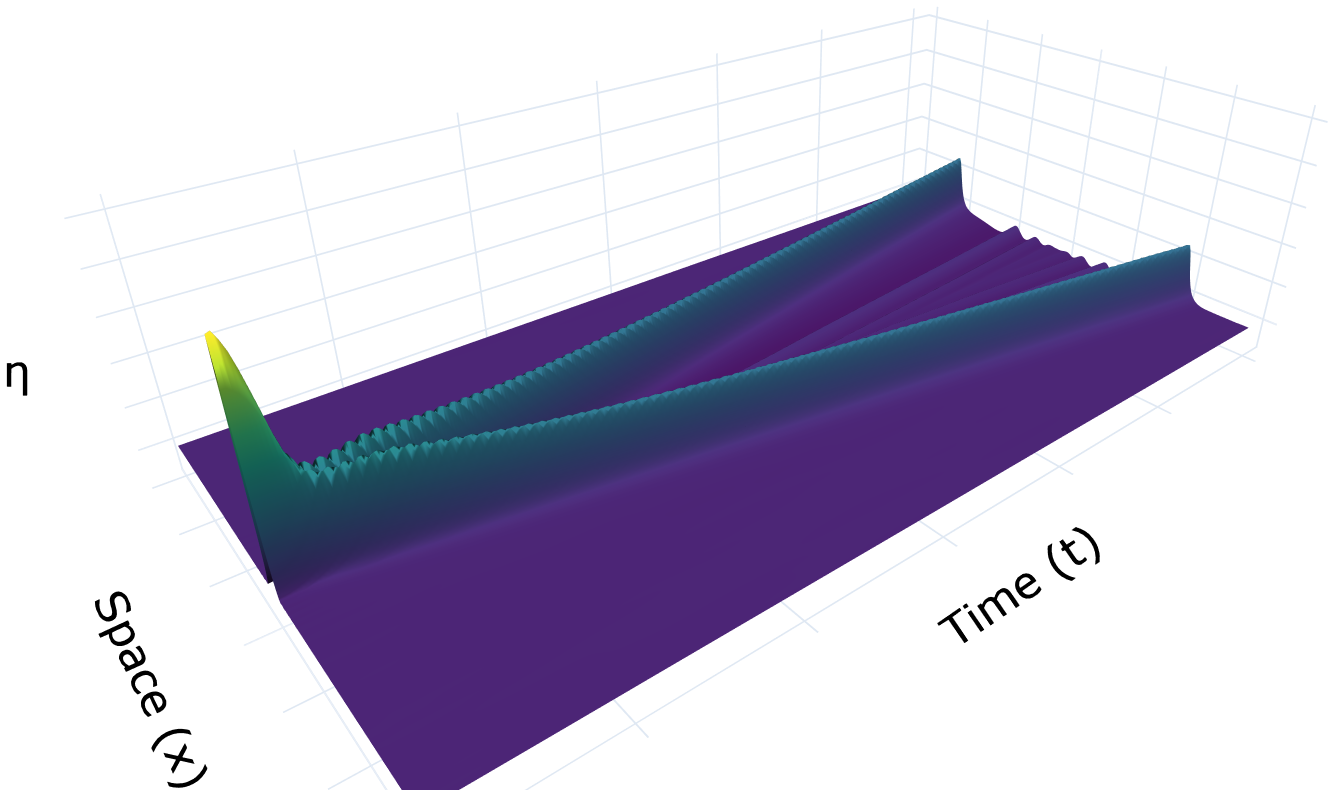
\includegraphics[width=\linewidth]{boussinesq_sciml/no/data_and_physics/pino_model2_alpha_beta_panel_surface_2.png}
        \end{minipage}\hfill
        \begin{minipage}[b]{0.49\linewidth}
          \centering
          {\small Erro relativo}\\[0.5ex]
          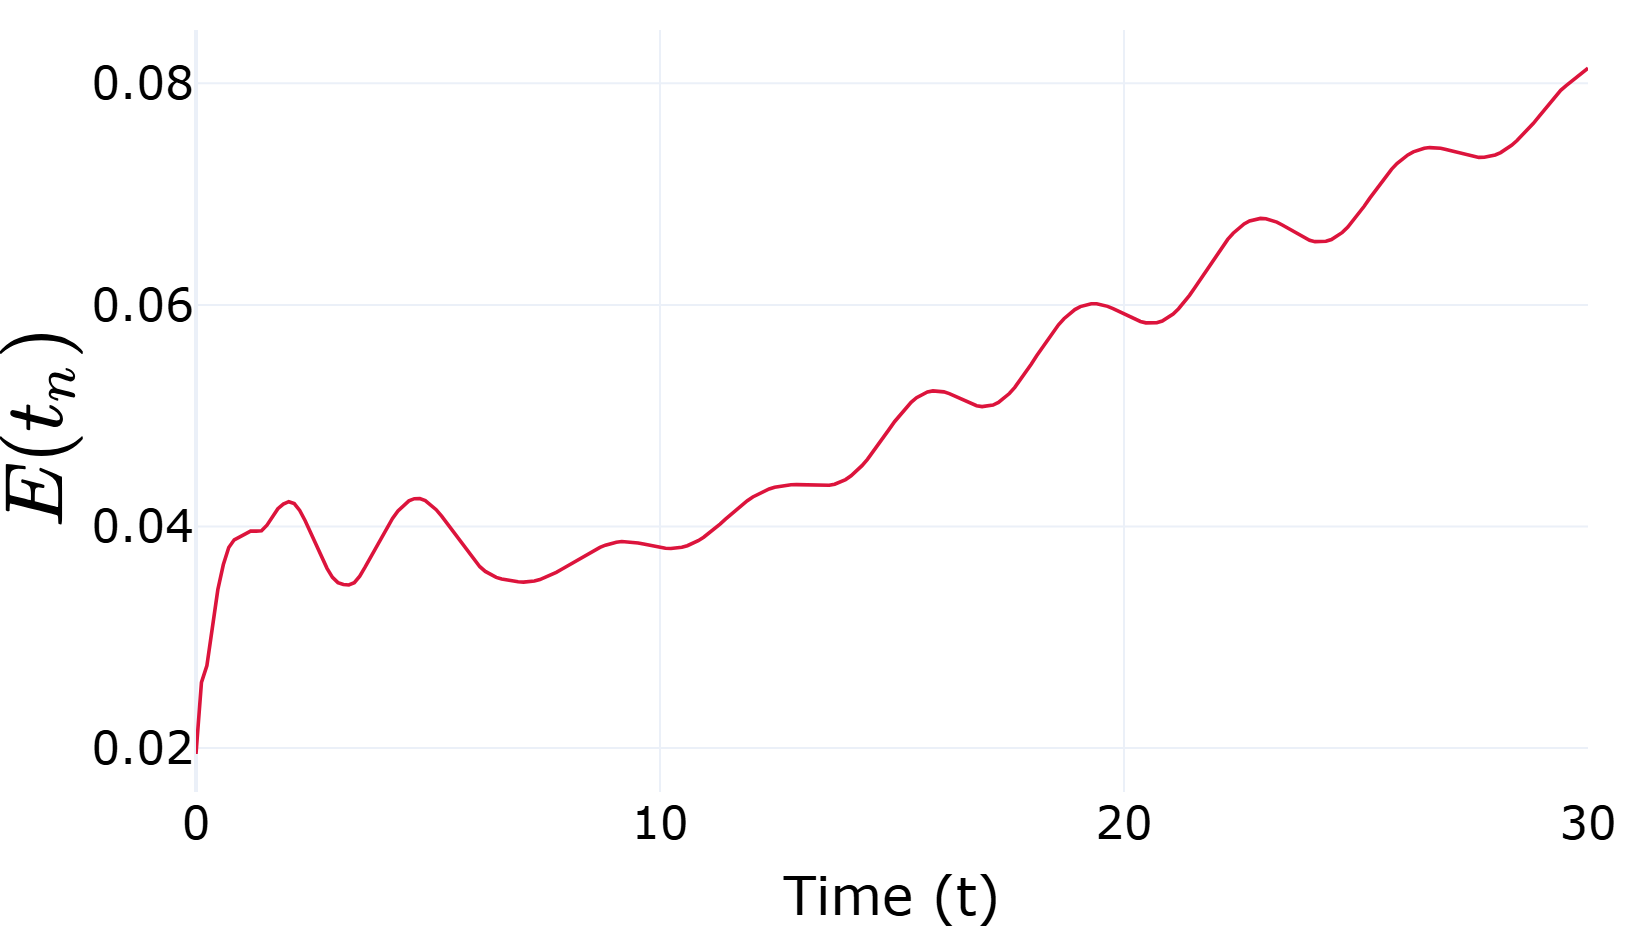
\includegraphics[width=\linewidth]{boussinesq_sciml/no/data_and_physics/pino_model2_alpha_beta_panel_relerr_2.png}
        \end{minipage}
        \caption{PINO (\textit{data and physics}) em $\alpha = \beta = 3{,}21$ e resolução $256$: elevação $\eta(x,t)$ prevista (esquerda) e erro relativo $E(t_n)$ em relação à referência pseudoespectral ao longo do tempo (direita).}
        \label{fig:pino}
      \end{figure}

      \heading{Viés espectral na previsão}
      O viés espectral também aparece no resultado final do PINO (\textit{data and physics}). No espectro da previsão (Figura~\ref{fig:espectro}), os modos baixos coincidem com os da referência, enquanto nos modos altos a amplitude prevista fica abaixo da amplitude de referência.

      \begin{figure}
        \centering
        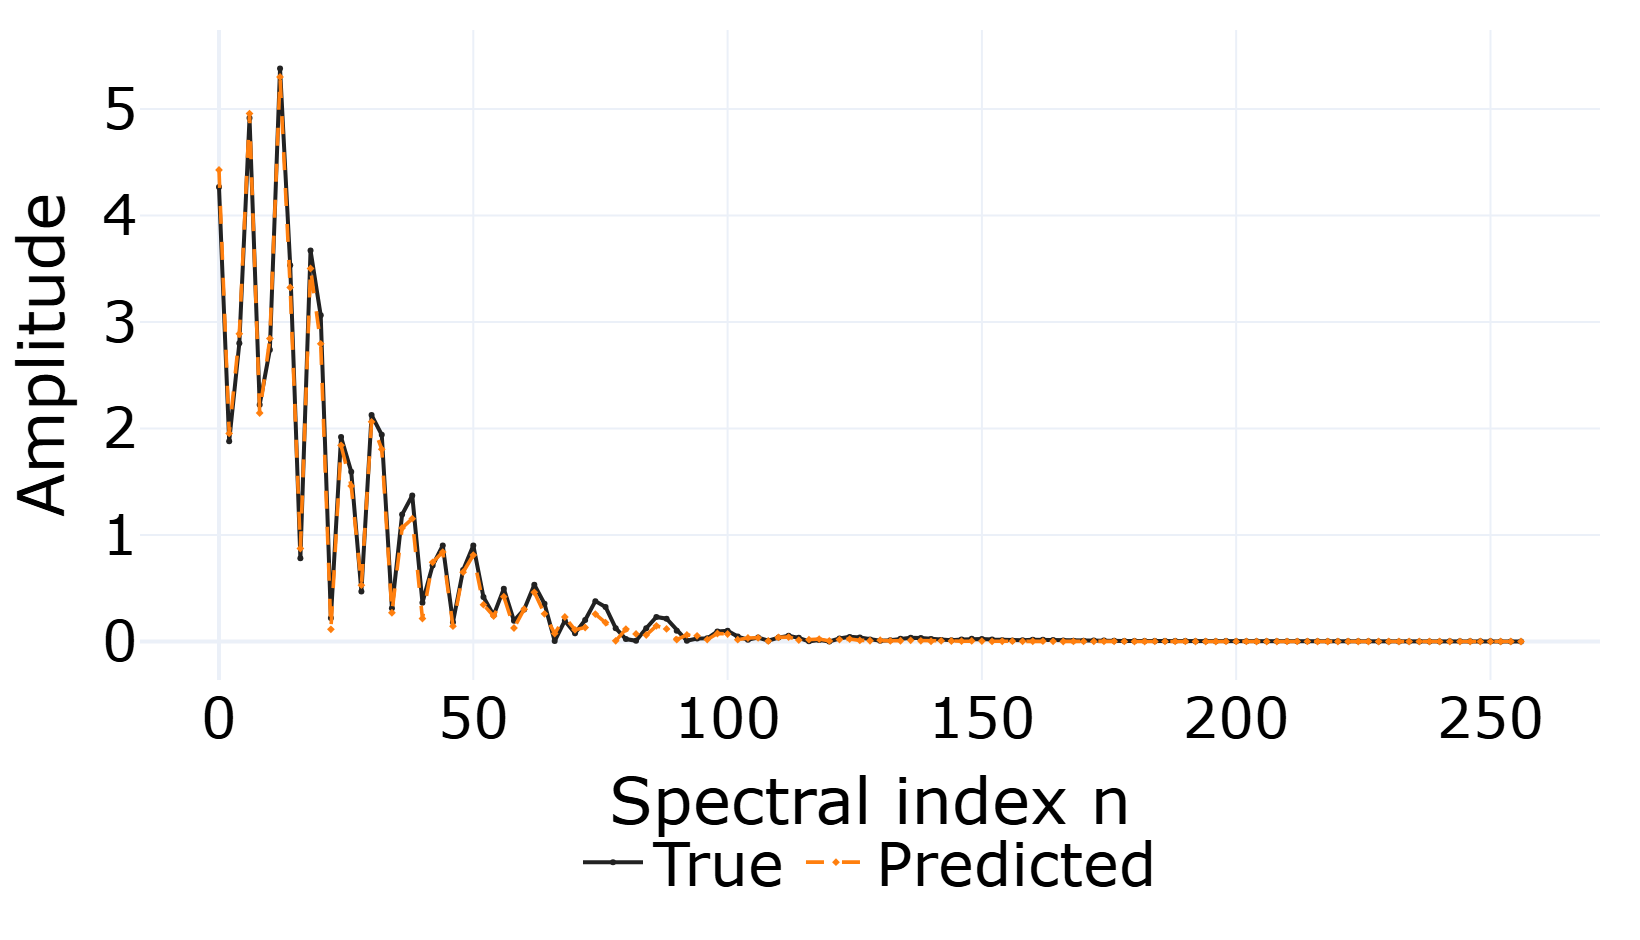
\includegraphics[width=0.66\linewidth]{boussinesq_sciml/no/data_and_physics/pino_model2_spectral_panel_spectrum_2.png}
        \caption{Espectro de $\eta$ em $t = 15$ para o PINO (\textit{data and physics}), em $\alpha = \beta = 3{,}21$ e resolução $256$: amplitude $|\hat\eta(k,t)|$ da referência (\textit{True}) e da previsão (\textit{Predicted}).}
        \label{fig:espectro}
      \end{figure}
  \end{plainblock}
\end{column}

\separatorcolumn

\begin{column}{\colwidth}
  \begin{plainblock}
      \heading{Viés espectral no treinamento}
      A Figura~\ref{fig:bandas} acompanha o erro por banda durante o treinamento dos três operadores, na amostra de treino mais próxima de $3{,}21$ ($\alpha = \beta \approx 3{,}18$) e na resolução de treinamento, $128$. Nos dois PINOs, o erro da banda baixa cai continuamente, o da banda média cai mais devagar e o da banda alta fica quase constante após as primeiras iterações. No FNO (\textit{pure data}), a banda baixa oscila durante todo o treinamento e a alta termina acima das outras duas. O PINO (\textit{pure physics}) termina com erro maior nas três bandas do que o PINO (\textit{data and physics}).

      \begin{figure}
        \centering
        \begin{minipage}[b]{0.49\linewidth}
          \centering
          {\small FNO (\textit{pure data})}\\[0.5ex]
          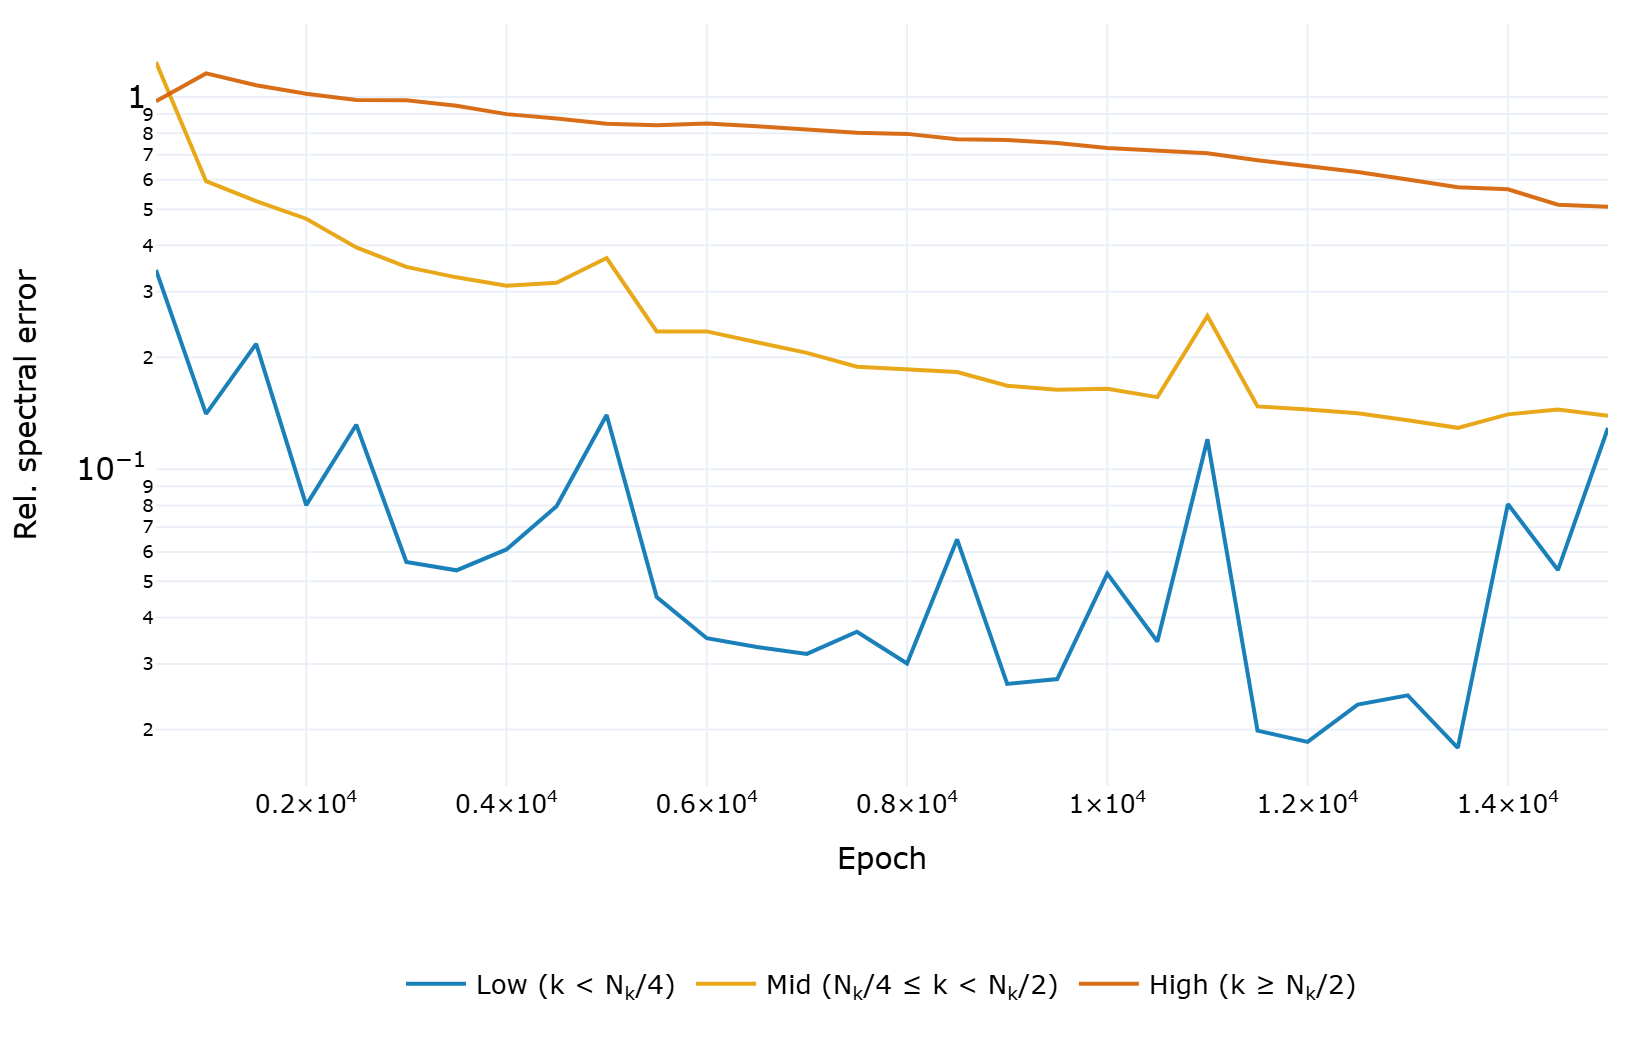
\includegraphics[width=\linewidth]{boussinesq_sciml/comparison/spectral_bias_evolution_fno_pure_data.png}
        \end{minipage}\hfill
        \begin{minipage}[b]{0.49\linewidth}
          \centering
          {\small PINO (\textit{data and physics})}\\[0.5ex]
          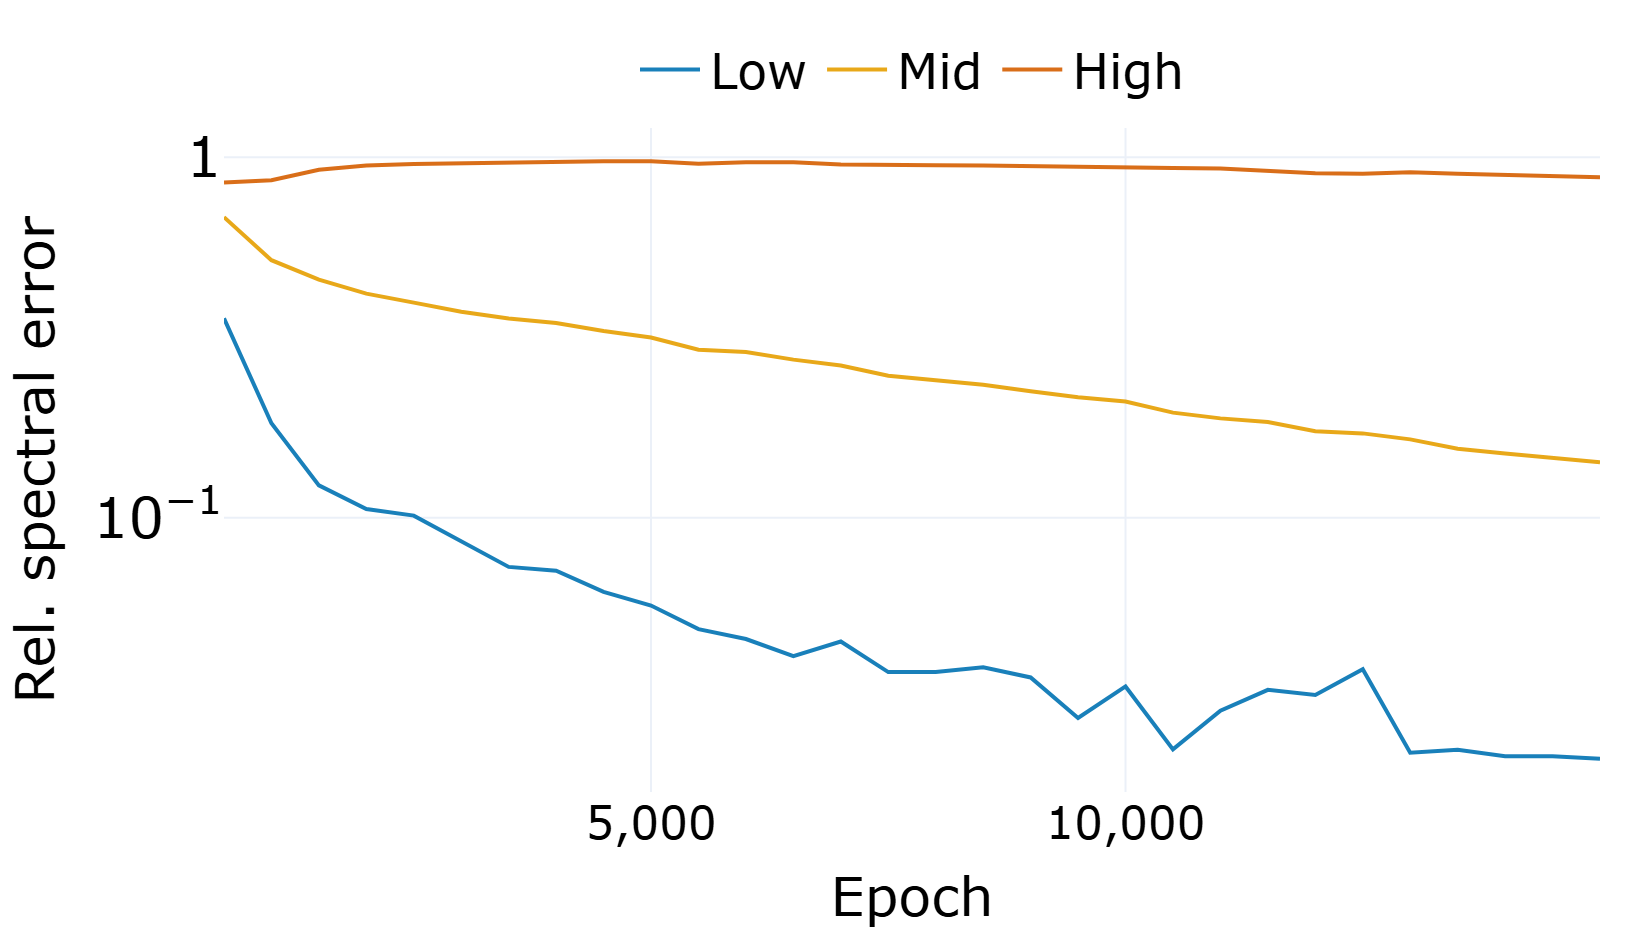
\includegraphics[width=\linewidth]{boussinesq_sciml/comparison/spectral_bias_evolution_pino_data_and_physics.png}
        \end{minipage}

        \vspace{1.5ex}
        \begin{minipage}[c]{0.49\linewidth}
          \centering
          {\small PINO (\textit{pure physics})}\\[0.5ex]
          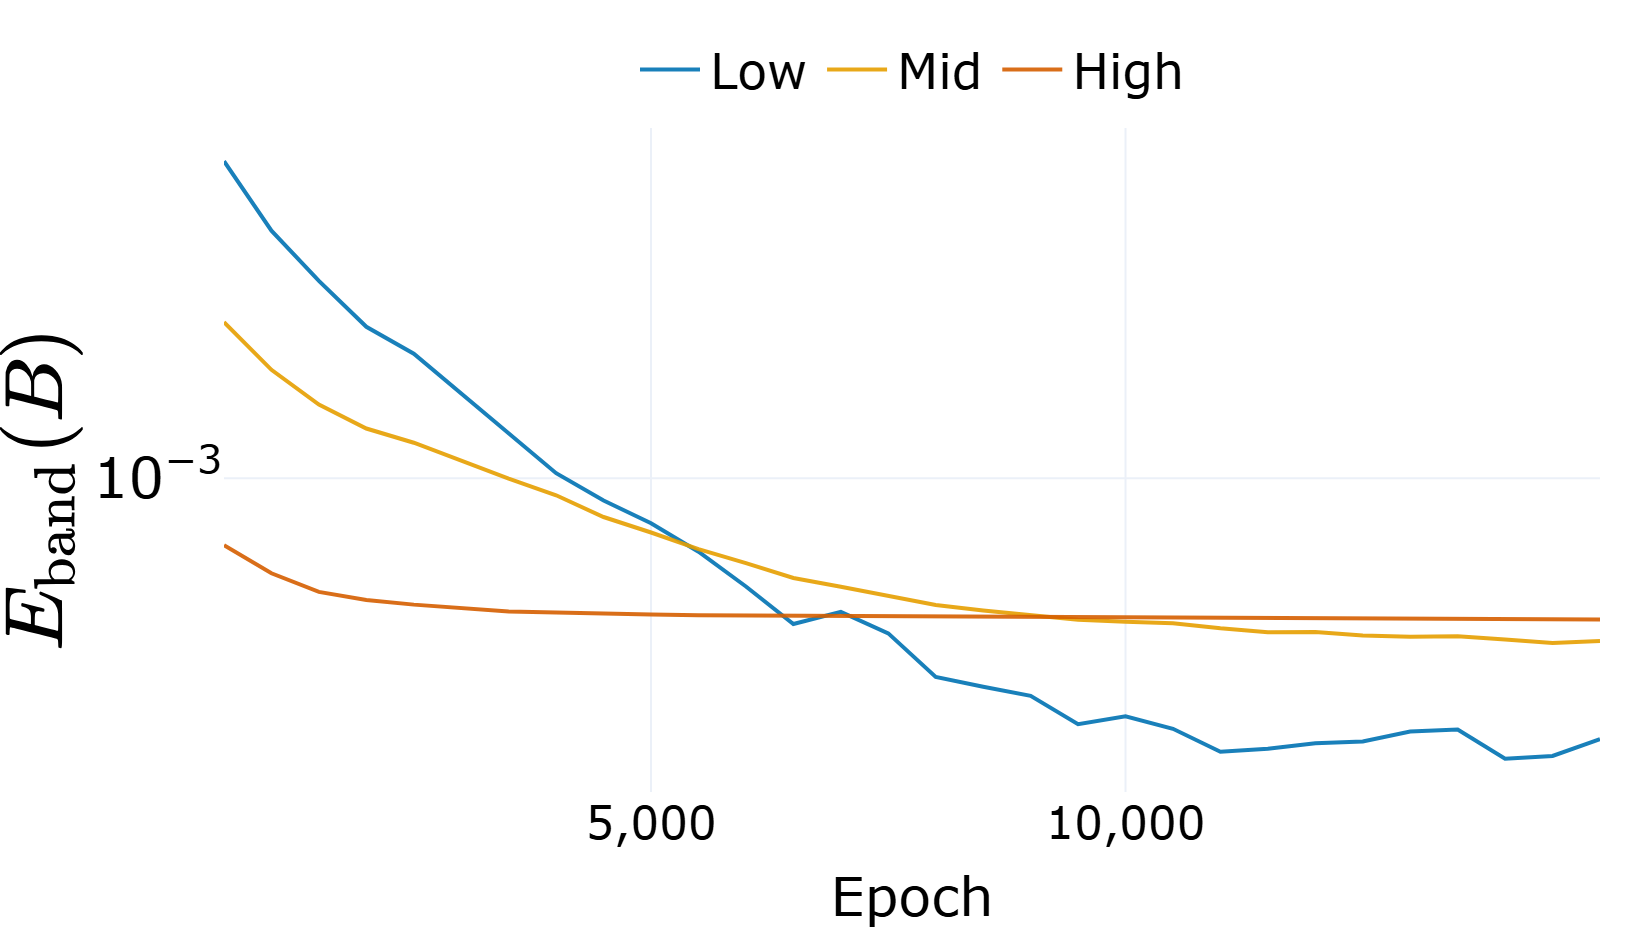
\includegraphics[width=\linewidth]{boussinesq_sciml/comparison/spectral_bias_evolution_pino_pure_physics.png}
        \end{minipage}\hfill
        \begin{minipage}[c]{0.46\linewidth}
          \caption{Erro espectral médio por banda, $E_{\text{band}}$, ao longo do treinamento, em $\alpha = \beta \approx 3{,}18$ e resolução $128$. \textit{Low}, \textit{Mid} e \textit{High} são as bandas baixa, média e alta; as escalas verticais diferem entre os painéis.}
          \label{fig:bandas}
        \end{minipage}
      \end{figure}
  \end{plainblock}

  \begin{block}{Conclusões}
    \begin{itemize}
      \item O viés espectral apareceu nos três operadores neurais: ao fim do treinamento, a banda alta concentrou o maior erro, e nos dois PINOs ela quase não mudou após as primeiras iterações.
      \item Com dados supervisionados, os operadores terminaram o treinamento com erro menor nas bandas baixa e média do que apenas com o resíduo da equação.
      \item A combinação de dados e física teve o menor erro relativo entre os métodos testados: o resíduo funcionou melhor como regularizador somado aos dados do que como substituto deles.
    \end{itemize}
    Esses métodos complementam o solucionador clássico, sem substituí-lo. Um operador treinado responde a uma varredura de parâmetros com uma passagem pela rede, mas é o solucionador pseudoespectral que fornece os dados de treinamento e a referência contra a qual eles são medidos.
  \end{block}

\end{column}

\separatorcolumn
\end{columns}

% ====================
% LINHA 3: referências, na largura inteira e em três colunas
% ====================
\begin{columns}[t]
\separatorcolumn

\begin{column}{\fullwidth}

  \begin{block}{Referências}
    \scriptsize
    \begin{multicols}{3}
    \begin{thebibliography}{9}
      \bibitem{karniadakis2021}
      Karniadakis, G. E., Kevrekidis, I. G., Lu, L., Perdikaris, P., Wang, S. e Yang, L. Physics-informed machine learning, \textit{Nature Reviews Physics}, 3:422--440, 2021. DOI: 10.1038/s42254-021-00314-5.

      \bibitem{li2021}
      Li, Z., Kovachki, N., Azizzadenesheli, K., Liu, B., Bhattacharya, K., Stuart, A. e Anandkumar, A. Fourier neural operator for parametric partial differential equations, \textit{International Conference on Learning Representations (ICLR)}, 2021.

      \bibitem{li2023pino}
      Li, Z., Zheng, H., Kovachki, N., Jin, D., Chen, H., Liu, B., Azizzadenesheli, K. e Anandkumar, A. Physics-informed neural operator for learning partial differential equations, \textit{ACM/IMS Journal of Data Science}, 1(3):1--27, 2024. DOI: 10.1145/3648506.

      \bibitem{martins2023}
      Martins, L. G. Estudo numérico do modelo Boussinesq com topografia e pressão variável no espaço e no tempo, Dissertação de Mestrado, UFPR, 2023.

      \bibitem{rahaman2019}
      Rahaman, N., Baratin, A., Arpit, D., Draxler, F., Lin, M., Hamprecht, F. A., Bengio, Y. e Courville, A. On the spectral bias of neural networks, \textit{Proceedings of the 36th International Conference on Machine Learning}, PMLR 97:5301--5310, 2019.

      \bibitem{raissi2019}
      Raissi, M., Perdikaris, P. e Karniadakis, G. E. Physics-informed neural networks: a deep learning framework for solving forward and inverse problems involving nonlinear partial differential equations, \textit{Journal of Computational Physics}, 378:686--707, 2019. DOI: 10.1016/j.jcp.2018.10.045.
    \end{thebibliography}
    \end{multicols}
  \end{block}

\end{column}

\separatorcolumn
\end{columns}

\end{frame}

\end{document}
